%% 
%% Copyright 2007, 2008, 2009 Elsevier Ltd
%% 
%% This file is part of the 'Elsarticle Bundle'.
%% ---------------------------------------------
%% 
%% It may be distributed under the conditions of the LaTeX Project Public
%% License, either version 1.2 of this license or (at your option) any
%% later version.  The latest version of this license is in
%%    http://www.latex-project.org/lppl.txt
%% and version 1.2 or later is part of all distributions of LaTeX
%% version 1999/12/01 or later.
%% 
%% The list of all files belonging to the 'Elsarticle Bundle' is
%% given in the file `manifest.txt'.
%% 

%% Template article for Elsevier's document class `elsarticle'
%% with numbered style bibliographic references
%% SP 2008/03/01

\documentclass[preprint,12pt]{elsarticle}
%\documentclass[final,1p,times]{elsarticle}
\usepackage{lineno,hyperref}
\modulolinenumbers[5]

%\usepackage[notref]{showkeys}

%% Use the option review to obtain double line spacing
%% \documentclass[authoryear,preprint,review,12pt]{elsarticle}

%% Use the options 1p,twocolumn; 3p; 3p,twocolumn; 5p; or 5p,twocolumn
%% for a journal layout:
%% \documentclass[final,1p,times]{elsarticle}
%% \documentclass[final,1p,times,twocolumn]{elsarticle}
%% \documentclass[final,3p,times]{elsarticle}
%% \documentclass[final,3p,times,twocolumn]{elsarticle}
%% \documentclass[final,5p,times]{elsarticle}
%% \documentclass[final,5p,times,twocolumn]{elsarticle}

%% For including figures, graphicx.sty has been loaded in
%% elsarticle.cls. If you prefer to use the old commands
%% please give \usepackage{epsfig}

%% The amssymb package provides various useful mathematical symbols
\usepackage{amssymb}

\usepackage{amsmath}
\usepackage{amsfonts}
\usepackage{amssymb}
\usepackage{bm}
%% The amsthm package provides extended theorem environments
% %\usepackage{amsthm}

%% The lineno packages adds line numbers. Start line numbering with
%% \begin{linenumbers}, end it with \end{linenumbers}. Or switch it on
%% for the whole article with \linenumbers.
%% \usepackage{lineno}


\newtheorem{thm}{Theorem}
\newtheorem{lem}[thm]{Lemma}
\newdefinition{rmk}{Remark}
\newproof{pf}{Proof}
\newproof{pot}{Proof of Theorem \ref{thm2}}
\DeclareMathOperator*{\argmin}{arg\,min}

%\newtheorem{thm}{{\sc Theorem}}[section]
\newtheorem{dfn}{{\sc Definition}}[section]
\newtheorem{prp}{{\sc Proposition}}[section]
\newtheorem{lm}{{\sc Lemma}}[section]
\newtheorem{cor}{{\sc Corollary}}[section]
\newtheorem{ex}{{\sc Example}}[section]

%\journal{Reliability Engineering \& System Safety}

%% `Elsevier LaTeX' style
\bibliographystyle{elsarticle-num}
%%%%%%%%%%%%%%%%%%%%%%%

\begin{document}
\begin{frontmatter}

%\title{Elsevier \LaTeX\ template\tnoteref{mytitlenote}}
\title{Evaluation of aging properties  by a scale-space inspection of the TTT curve\tnoteref{title1}}

%\tnotetext[mytitlenote]{Fully documented templates are available in the elsarticle package on \href{http://www.ctan.org/tex-archive/macros/latex/contrib/elsarticle}{CTAN}.}

%% Group authors per affiliation:
%% Group authors per affiliation:
\author{G\'amiz, M.L.\fnref{myfootnote}}
\fntext[myfootnote]{Corresponding author}
\ead{mgamiz@ugr.es}

\author{Nozal-Ca\~nadas, R.}
\author{ Raya-Miranda, R.}

\address{University of Granada}
%
%% or include affiliations in footnotes:
%\author[mymainaddress,mysecondaryaddress]{Elsevier Inc}
%\ead[url]{www.elsevier.com}
%
%\author[mysecondaryaddress]{Global Customer Service\corref{mycorrespondingauthor}}
%\cortext[mycorrespondingauthor]{Corresponding author}
%\ead{support@elsevier.com}

%\address[mymainaddress]{Dept. of Statistics and O.R.}
%\address[mysecondaryaddress]{360 Park Avenue South, New York}
%\ead{mgamiz@ugr.es}

\begin{abstract}
This template helps you to create a properly formatted \LaTeX\ manuscript.
\end{abstract}

\begin{keyword}
Total-Tim-on-Test Transform \sep Kernel smoothing \sep Order statistics \sep SiZer map
\MSC[2010] 90B25 \sep  62N05
\end{keyword}

\end{frontmatter}

\linenumbers

\bigskip

\section{Introduction}
In many applications (e.g. reliability, maintainability, biometry or survival) different forms of aging are of interest giving rise to a well-known nonparametric classification of life distributions (Barlow and Proschan, 1975). While  ``positive aging'' describes the adverse effects of age on the lifetime of components or systems and describes the situation where the residual life tends to decrease in some probabilistic sense with increasing age,  ``no aging'' means that age has no effect on residual life of an item, and  ``negative agin'' means that the item experiences certain improvement in performance or reliability with age, see Lay {\it et al.} (2006). We are concerned with ``positive aging''  however it has to be mentioned that the classification according to different types of ``positive aging'' has a parallel in terms of ``negative aging''.

%As we know the notion of aging plays an important role in reliability and survival theory and in a technical context, 
In a technical contex, aging is usually understood as a gradual decrease in performance over time, so it can be expected that the aging of a component or system increases the probability that it will fail. 

If the lifetime of a mechanism is a random variable $ X $, a natural measure of aging could be the probability of surviving above $ t + x $, assuming that the mechanism has an age of at least $ t $, this idea leads to the concept of residual life that will be formally defined later in this paper.
Another possible measure of aging is formulated in terms of the hazard function, which measures the  instantaneous propensity to the failure of a mechanism as a function of  its age. An inspection of the shape of these functions is very useful to evaluate the performance of a system in the future which is very important for making decisions in maintainability and inventory theory, for example. 
%In this sense, to identify a life distribution with a particular type of aging and then to establish a classification of families of random variables according to the concept of aging is very useful when performing  reliability and maintenance analyses of physical mechanisms.

 The most usual classes of life distributions are denoted in the literature as IFR, IFRA, NBU, NBUE and DMRL  (with duals) and can be found in Barlow and Proschan (1975), Kochar and Singh (1988) and Cao and Wang (1991), among others.
 Although, the mathematical description of aging is done under three broad categories based on hazard functions, residual life functions and survival functions, in this paper we will look at the Total-Time-on-Test curve (TTT) and we will construct a useful and novel graphical tool to characterize some important types of aging.  The TTT plot was introduced by Barlow and Campo (1975) as a tool for analysing failure data and thus some important classes of life distributions (see Bergman and Klefsjo, 1983) are characterized in terms of the Total-Time-on-Test curve. Let us now to introduce some notation and relevant definitions. Let $X$ denote a random lifetime with absolutely continuous distribution function. 

\begin{dfn} {\bf Residual life}

\noindent Let $X$ a lifetime with survival function $S$, for any fixed $t>0$ we denote $X_t$ the residual lifetime from time $t$, which represent the additional lifetime from $t$. The conditional survival function is obtained as $S_t(x)=S(t+x)/S(t)$, for all $x >0$. The mean residual time is then defined as $\mu_t= \int_0^{+\infty} \frac{S(t+x)}{S(t)}dx$.
\end{dfn}


\begin{dfn} {\bf Aging classes}

\noindent Let $X$ be a lifetime with distribution function $F$, survival function $S$ and finite mean $\mu$.

\begin{enumerate}
\item Increasing (decreasing) failure rate, $IFR(DFR)$:

\noindent $X$ is {\it IFR}({\it DFR}) if and only if its conditional survival function is increasing (decreasing). That is, for all $x>0 $ fixed, and for all $t_1 < t_2$ we have that $S_{t_1}(x) \leq (\geq) S_{t_2}(x) $. This condition can be also stablished in terms of the hazard rate, saying that $X$ is {\it IFR}({\it DFR}) its hazard function is increasing (resp. decreasing).

\item Upside-down Failure Rate, $UFR$:
\noindent $X$ is {\it UFR}  if and only if its hazard function is initially increasing to a pick after declining abruptly till stabilize.

\item Bathtub shaped Failure Rate, $BFR$:
\noindent $X$ is  ({\it BFR}) if and only if its  hazard rate curve is divided into three regions: decreasing hazard rate region, constant hazard rate region, and increasing hazard rate region.

\item Decreasing (increasing) mean residual life, $DMRL(IMRL)$:

 \noindent $X$ is {\it DMRL}({\it IMRL}) if and only if $\mu_t$ is decreasing (increasing) for all $t>0$.

\item New better (worse) than used in expectation, $NBUE(NWUE)$:

 \noindent $X$  is {\it NBUE} ({\it NWUE}) if and only if  $\mu_t \leq (\geq) \mu$, for all $t>0$; where $\mu_t=\int_0^{+\infty}\frac{S(t+x)}{S(t)}dx$, denotes the expected residual life of a mechanism with distribution $F$ and at the age $t$.

\end{enumerate}
\end{dfn}

%\noindent Some important classes of life distributions (see Bergman and Klefsjo, 1983) can be characterized in terms of the Total-Time-on-Test curve. We recall some of the most well-known classes but first we need the following definition. We assume that $X$ is a random lifetime with absolutely continuous distribution function. 
%
%\begin{dfn} {\bf Residual life}
%
%\noindent Let $X$ a lifetime with survival function $S$, for any fixed $t>0$ we denote $X_t$ the residual lifetime from time $t$, which represent the additional lifetime from $t$. The conditional survival function is obtained as $S_t(x)=S(t+x)/S(t)$, for all $x >0$. The mean residual time is then defined as $\mu_t= \int_0^{+\infty} \frac{S(t+x)}{S(t)}dx$.
%\end{dfn}
%
%
%\begin{dfn} {\bf Aging classes}
%
%\noindent Let $X$ be a lifetime with distribution function $F$, survival function $S$ and finite mean $\mu$.
%
%\begin{enumerate}
%\item Increasing (decreasing) failure rate, $IFR(DFR)$:
%
%\noindent $X$ is {\it IFR}({\it DFR}) if and only if its conditional survival function is increasing (decreasing). That is, for all $x>0 $ fixed, and for all $t_1 < t_2$ we have that $S_{t_1}(x) \leq (\geq) S_{t_2}(x) $. This condition can be also stablished in terms of the hazard rate, saying that $X$ is {\it IFR}({\it DFR}) its hazard function is increasing (resp. decreasing).
%
%\item Upside-down Failure Rate, $UFR$:
%\noindent $X$ is {\it UFR}  if and only if its hazard function is initially increasing to a pick after declining abruptly till stabilize.
%
%\item Bathtub shaped Failure Rate, $BFR$:
%\noindent $X$ is  ({\it BFR}) if and only if its  hazard rate curve is divided into three regions: decreasing hazard rate region, constant hazard rate region, and increasing hazard rate region.
%
%\item Decreasing (increasing) mean residual life, $DMRL(IMRL)$:
%
 %\noindent $X$ is {\it DMRL}({\it IMRL}) if and only if $\mu_t$ is decreasing (increasing) for all $t>0$.
%
%\item New better (worse) than used in expectation, $NBUE(NWUE)$:
%
 %\noindent $X$  is {\it NBUE} ({\it NWUE}) if and only if  $\mu_t \leq (\geq) \mu$, for all $t>0$; where $\mu_t=\int_0^{+\infty}\frac{S(t+x)}{S(t)}dx$, denotes the expected residual life of a mechanism with distribution $F$ and at the age $t$.
%
%\end{enumerate}
%\end{dfn}


Parts of the paper:
\begin{itemize}
\item Definition and properties of the Total-Time-on-Test (TTT) transform
\item Local-polynomial fit of the TTT curve and its derivatives
\item SiZer map for studying convexity properties of a curve.
\item SiZer map for other aging properties
\item Hypothesis testing 
\end{itemize}

\section{Total-Time-on-Test transform: Definition and relevant properties} \label{sec:TTT}




\subsection{Definition of TTT curve}\label{sec:TTTdef}

\noindent Total time on test plots provide a useful graphical method for tentative identification of lifetime models. This concept is very important in applications in reliability analysis. When several units are tested for studying their life lengths some of the units would fail while others may survive the test period. The sum of all observed and incomplete life lengths is the total time on test statistics. The plot of this statistic versus time is called the total-time-on-test plot. As the number of units on test tends to infinity the limit of this statistic is called the total time on test transform (TTT). This concept was introduced by \cite{BD1900} and later studied by \cite{BP75}.
Model identification is based on properties of the TTT transform. 

\begin{dfn} \textbf{Total-Time-on-Test statistic} \label{ttt.def1}

\noindent Suppose $n$ items under test and successive failures are observed at $0=X_{(0)} \leq X_{(1)} \leq X_{(2)}\leq \cdots \leq X_{(n)}$, with $X_{(i)}$ the $i$-th order statistic from a lifetime random variable $X$ with absolutely continuous distribution function $F$. Then the \textit{total time on test statistic} during the interval $(0,t)$ is defined as 
\[
\tau (t) = \sum_{i=1}^r X_{(i)}+\left(n-r\right)t,
\]
provided that $X_{(r-1)}<t\leq X_{(r)}$.

\end{dfn}

For comparison purposes, usually the statistic is scaled to the interval $[0,1]$ by means of the transformation $\tau\left(X_{(r)}\right)/\tau\left(X_{(n)}\right)$, for $r=1,2,\ldots,n$.

Based on the sample order statistics we can construct the empirical distribution function, that is $F_n(t)=r/n$, for $X_{(r)} \leq t < X_{(r+1)}$, for $r=1,2,\ldots,n-1$; with $F_n(t)=0$, for $t <X_{(1)}$; and, with $F_n(t)=1$, for $t \geq X_{(n)}$. We can define the following function
\[
F^{-1}_n(p)= \inf \left\{x \geq 0:F_n(x) >p\right\},
\]
it can be checked, Nair {\it et al.} (2010), that
\[
\int_0^{F^{-1}_n\left(\frac{r}{n}\right)} \left(1-F_n(t)\right)dt= \frac{\tau\left(X_{(r)}\right)}{n},
\]
and also that
\[
\underset{n\rightarrow \infty}{\lim}\underset{\frac{r}{n}\rightarrow p}{\lim}\int_0^{F^{-1}_n\left(\frac{r}{n}\right)}\left(1-F_n(t)\right) dt= \int_0^{F^{-1}(p)}\left(1-F(t)\right) dt,
\]
uniformly in $p\in (0,1)$. 

\begin{dfn}\textbf{Total Time on Test transform} \label{ttt.def2} 

\noindent Let $X$ be a (non-negative) random variable with absolutely continuous cumulative distribution function $F$. The \textit{total time on test transform} of $X$ is defined as
\begin{equation} \label{ttt.curve}
\varphi(p) =\int_0^{Q(p)}\left(1-F(t)\right) dt
\end{equation}
where we denote $Q(p)= F^{-1}(p)$, for $p\in [0,1]$, the corresponding quantile function.
\end{dfn}
When $E[X] < \infty$, this expectation can be obtained as $\mu=\int_0^{Q(1)} S(t)dt$, where we denote $S(t)=1-F(t)$, the survival function. Then we define the \textbf{\textit{scaled}} TTT transform as $\varphi(p)/\mu$, for $0 \leq p \leq 1$,  which is scale invariant. We keep notation $\varphi(p)$ for the scaled TTT transform, and we assume that $\mu=1$, since it does not imply any loss of generality.


\subsection{Aging properties based on the TTT transform}\label{sec:aging}


\noindent The scaled TTT transform can be used to characterize different aging properties, see Barlow and Proschan, (1975) and Bergman and Lindqvist (1983). For $F$ the exponential distribution, it can be checked that $\varphi(p)=p$, for $0 \leq p \leq 1$. As mentioned above, based on a sample $X_1,X_2,\ldots, X_n$ one can construct the TTT plot, which will be closer to the scaled TTT curve as $n$ tends to $+\infty$. We can thus use the TTT plot as a tool for model selection, in the sense that when, for example, the TTT plot produces a cloud of points around the diagonal of the square unit, we can admit that the distribution of the underlying lifetime $F$ is exponential, that is with constant hazard rate. Other hazard shapes can be recognized from an inspection of the TTT plot. A convex TTT curve corresponds with a decreasing hazard (DFR); a concave TTT curve corresponds with an increasing hazard (IFR). When the TTT plot describes a trajectory first convex then concave it indicates a bathtub hazard shape and when it is concave then convex, it indicates a unimodal hazard shape. 

In summary, to determine the type of aging represented by $X$ we can study the shape of the TTT curve. To do it we compute the first and second derivatives of the TTT transform. Using expression \eqref{ttt.curve} can be obtained as
\begin{eqnarray*}
\varphi'(p)&=& \frac{d}{d p}\left\{\int_0^{Q(p)}S(x)dx\right\}=S\left(Q(p)\right)Q'(p)=(1-p)Q'(p); \ {\rm and}, \\
\varphi''(p)&=& -Q'(p)+(1-p)Q''(p). 
\end{eqnarray*}
where $Q'(p)=dQ(p)/dp$ and $Q''(p)=d^2Q(p)/d^2p$.

%\begin{ex}\label{expon}{Exponential distribution}
%Let $X$ be a random variable with distribution $Exp(\lambda)$.....
%\end{ex}



Let $X$ be a lifetime with distribution function $F$ and with finite mean $\mu$. From the theorems given in Klefsjo (1980) the above aging conditions can be expressed in terms of the TTT-curve as follows
\begin{prp} {TTT-curve characterization of aging} \

\begin{enumerate}
\item $ F$ is $ IFR(DFR)$ if and only if $ \varphi'' (u) \leq (\geq) 0$, for all $0 <u <1$;
\item $F$ is $DMRL(IMRL)$ if and only if $ \varphi'(u) \leq (\geq) \frac{1-\varphi(u)}{1-u}$;
\item $F$ is $ NBUE(NWUE)$ if and only if $\varphi(u)/u \leq (\geq) 1$, for all $0 <u <1$.

\end{enumerate}
 \end{prp}
%%%%%%%%%%%%%%%%%%%%%%%%%%%%%%%%%%%%%%%%%%%%%%%%%%%%%%%%%%%%%%%%%%%%%%%%%%%%%
%%%%%%%%%%%%%%%%%%%%%%%%%%%%%%%%%%%%%%%%%%%%%%%%%%%%%%%%%%%%%%%%%%%%%%%%%%%%%
%\section{Kernel estimation of the TTT curve and its first and second derivatives based on quantile estimation}
%**** ESTA SECCION SE ELIMINARA EN LA VERSION FINAL****
%
%We consider to estimate the TTT curve and its derivatives through nonparametric kernel estimation techniques. To obtain the estimator of these curves we need to conveniently estimate the quantile function. We distinguish two cases: $iid$ data and $censored$ data.
%
%\subsection{Kernel estimation of quantiles with $iid$ samples}
%Let $X_1,X_2,\cdots,X_n$ be an independent and identically distributed random sample drawn form an absolutely continuous distribution function $F$ with density $f$. Let $X_{(1)},X_{(2)},\cdots,X_{(n)}$ denote the corresponding order statistics. The quantile function $Q$ of the population is defined as $Q(p)=\inf \left\{x: F(x) \geq p\right\}$, $0<p<p$. The classical nonparametric estimator of $F$ is the empirical cumulative distribution function (ecdf) $F_n(t)=n^{-1}\sum_{i=1}^n I\left\{X_{(i)}\leq t\right\}$. The simplest method to estimate the quantile function is the empirical quantile estimator, that is $Q_n(p)=\inf \left\{x: F_n(x) \geq p\right\}$, then in particular we have that $Q_n\left(\frac{i}{n}\right)=X_{(i)}$, for $i=1,2,\ldots, n$. Parzen () developed kernel smoothing on the empirical quantile leading to the kernel quantile estimator
%\begin{equation}\label{kernel.Q1}
%\widehat{Q}_h(p)=\int_0^1 Q_n(u)K_h(u-p)du
%\end{equation}
%where we define $K_h(\cdot)=K(\cdot/h)/h$, for $K$ a kernel function, and $h$ a smoothing parameter. We can approximate the kernel quantile in $(\ref{kernel.Q1})$ by
%\begin{equation}\label{kernel.Q2}
%\widehat{Q}_h(p)=\sum_{i=1}^n X_{(i)}\left\{\textbf{K}\left(\frac{\frac{i}{n}-p}{h}\right)-\textbf{K}\left(\frac{\frac{i-1}{n}-p}{h}\right)\right\}
%\end{equation}
%with ${\bf K} (u) =\int_{-\infty}^u K(s)ds$. From the expression in $(\ref{kernel.Q2})$ we can obtain the corresponding kernel estimators of the first and second derivatives of the quantile function as
%\begin{equation}\label{kernel.dQ}
%\widehat{Q}'_h(p)=\sum_{i=1}^n X_{(i)}\left\{K_h\left(\frac{i-1}{n}-p\right)-K_h\left(\frac{i}{n}-p\right)\right\}=\sum_{i=1}^n A_iX_{(i)};
%\end{equation}
%and,
%\begin{equation}\label{kernel.d2Q}
%\widehat{Q}''_h(p)=h^{-2}\sum_{i=1}^n X_{(i)}\left\{K'\left(\frac{\frac{i}{n}-p}{h}\right)-K'\left(\frac{\frac{i-1}{n}-p}{h}\right)\right\}=\sum_{i=1}^n B_iX_{(i)}.
%\end{equation}
%Now we plug-in these estimates in the expression of the second derivative of the TTT transform to define
%\begin{equation}\label{phi.2.1}
%\widehat{\varphi}''_h(p)=-\widehat{Q}'_h(p)+(1-p)\widehat{Q}''_h(p)
%\end{equation}
%So we can write the estimator in equation $(\ref{phi.2.1})$ as a linear combination of order statistics in the form
%\begin{equation}\label{phi.2.2}
%\widehat{\varphi}''_h(p)=\sum_{i=1}^n C_iX_{(i)}
%\end{equation}
%where $C_i=-A_i+(1-p)B_i$.
%The variance of the estimator can be obtained as
%\begin{equation}\label{var.phi}
%{\rm Var}\left(\varphi''_h(p)\right)=\sum_{i=1}^nC_i^2 {\rm Var}\left(X_{(i)}\right)+2\underset{i<j}{\sum}C_iC_j{\rm Cov}\left(X_{(i)},X_{(j)}\right)
%\end{equation}
%
%
%
%\subsection{Kernel estimation of quantiles with $censored$ data}
%***This section has to be developed****

%\newpage
%
\section{Local polynomial estimation of the TTT curve and its first and second derivatives}
%\subsection{Least-squares estimation of the Total-Time-on-Test transform with $iid$ samples} 
\noindent In this section we suggest a local-polynomial estimator for the TTT-transform directly formulated from an empirical estimation of the TTT-curve, that is, we do not need to estimate the quantiles to get an estimator of the TTT-transform.
%
\subsection{Least-squares estimation of the Total-Time-on-Test transform}
\noindent Let $X_1,X_2,\cdots,X_n$ be an independent and identically distributed random sample drawn form an absolutely continuous distribution function $F$ with density $f$. Let $X_{(1)},X_{(2)},\cdots,X_{(n)}$ denote the corresponding order statistics. Let us denote $p_i=\frac{i}{n}$ for $i= 1,2, \ldots, n$. An empirical ($naive$) estimator of the TTT-curve $\widehat{\varphi}_n$, can be defined as follows
%
\begin{equation}\label{empi}
\widehat{\varphi}_n\left(p_i\right)= \sum_{j=1}^i \left(1-\frac{j-1}{n}\right) \left(X_{(j)}-X_{(j-1)}\right),
\end{equation}
for $i=1,2,\ldots,n$, with $\widehat{\varphi}_n(0)=0$. We can observe that $\widehat{\varphi}_n(1)=\bar{X}$, the mean sample statistics. Since the properties of the curve are not affected by scale changes, we can confine the curve to be defined in the interval $[0,1]$ by first normalizing the data. That is, we work with the sample $\{X_i/\bar{X}; i=1,\ldots,n\}$. In the following, without loss of generality, we assume that $\bar{X}=1$.

Under a local-polynomial approach we consider that, for each estimation point $p_0 \in (0,1)$, the TTT-transform $\varphi(p_0)$ is locally (in a neighborhood of $p_0$) approximated by a $m$th-degree polynomial function in the sense that for all $p \in \left(p_0-h,p_0+h\right)$ we have that $\varphi(p)=\theta_0+\theta_1(p-p_0)+\theta_2(p-p_0)^2+\ldots+\theta_m(p-p_0)^m$, for an appropriate bandwidth $h$. 

The parameters of the model can be interpreted respectively as $\theta_0={\varphi}(p_0)$; ${\theta}_1={\varphi'}(p_0)$; and, in general, ${\theta}_k=\frac{\varphi^{(k)}(p_0)}{k!}$, for $k=1,2,\ldots,m$. The approximation above is valid locally if we assume certain smoothness conditions on the quantile function, in the sense of derivability. 


In particular, the three first coefficients provide the following estimates: $\widehat{\varphi}(p_0)=\widehat{\theta}$, $\widehat{\varphi'}(p_0)=\widehat{\theta}_1$, and $\widehat{\varphi''}(p_0)=2\widehat{\theta}_2$, respectively.
To this goal, we formulate the following least squares problem

\begin{eqnarray}\label{LS}
&&\left(\widehat{\theta}_0,\widehat{\theta}_1,\ldots,\widehat{\theta}_m\right)^{\intercal}= \\
\nonumber &&\underset{\left({\theta}_0,\theta_1,\ldots, {\theta}_m\right)^{\intercal}}{\arg \min} \sum_{i=1}^n\left\{\widehat{\varphi}_n(p_i)-\theta_0-\theta_1(p_i-p_0)-\ldots-\theta_m(p_i-p_0)^m\right\}^2 K_h(p_i-p_0),
\end{eqnarray}
where $K_h(\cdot)=\frac{1}{h}K(\frac{\cdot}{h})$, with $K$ a symmetric kernel function, and $h$ the bandwidth parameter that controls the size of the window around the estimation point $p_0$ where the polynomial approximation is valid.
After differentiating in equation ($\ref{LS}$), for $m=2$ with respect to $\theta_j$ ($j=0, 1, 2$), we obtain a system of linear equations that can be written in matrix form
\[
\left(\begin{array}{cccc}
a_0 & a_1&\cdots &a_m \\ 
a_{1} & a_2&\cdots &a_{m+1}\\
\vdots & \vdots &\ddots &\vdots \\ 
a_m & a_{m+1}&\cdots &a_{2 m} 
\end{array}\right)
\left(\begin{array}{c}
 \theta_0 \\ 
\theta_1 \\ 
\vdots \\
\theta_m
 \end{array}\right)=
\left(\begin{array}{c} 
A_0 \\ 
A_1 \\ 
\vdots \\
A_m
 \end{array}\right);
\]

where we have denoted

\[
A_r(p_0)=\sum_{i=1}^n\widehat{\varphi}_n(p_i)(p_i-p_0)^r K_h(p_i-p_0), \ \ r=0, \ 1,\ldots  m;
\]
and 
\[
a_l(p_0)=\sum_{i=1}^n(p_i-p_0)^l K_h(p_i-p_0), \ \ l=0,\ 1, \ 2, \ldots, 2m.
\]

\subsection{Local-quadratic estimator}\label{quad}
\noindent In particular we can fit the data locally by using a 2-degree polynomial. We denote this estimator $\widehat{\varphi}_{2,h}(\cdot)$. Then, we set the least squares problem of ($\ref{LS}$) for $m=2$ and define 
\[
A_r(p_0)=\sum_{i=1}^n\widehat{\varphi}_n(p_i)(p_i-p_0)^r K_h(p_i-p_0), \ \ r=0, \ 1, \ 2;
\]
and 
\[
a_l(p_0)=\sum_{i=1}^n(p_i-p_0)^l K_h(p_i-p_0), \ \ l=0,\ 1, \ 2, \ 3, \ 4.
\]
After differentiating in equation ($\ref{LS}$), for $m=2$ with respect to $\theta_j$ ($j=0, 1, 2$), we obtain a system of linear equations that can be written in matrix form
\begin{equation}\label{score}
\left(\begin{array}{c} 
A_0 \\ 
A_1 \\ 
A_2
 \end{array}\right)
=\left(\begin{array}{ccc}
a_0 & a_1 &a_2 \\ 
a_1 & a_2 &a_3 \\ 
a_2 & a_3 &a_4 
\end{array}\right)
\left(\begin{array}{c}
 \theta_0 \\ 
\theta_1 \\ 
\theta_2
 \end{array}\right).
\end{equation}
Using  Cramer's rule, the solution can be then expressed as
\[
\widehat{\theta}_0=\frac{\left|
\begin{array}{ccc} 
A_0 & a_1 &a_2 \\ 
A_1 & a_2 &a_3 \\ 
A_2 & a_3 &a_4
 \end{array}\right|}
 {\left|\begin{array}{ccc} 
a_0 & a_1 &a_2 \\
 a_1 & a_2 &a_3 \\
 a_2 & a_3 &a_4
 \end{array}\right|}=\widehat{\varphi}_h(p_0),
\hspace{0.5cm}
\widehat{\theta}_1=\frac{\left|
\begin{array}{ccc} 
a_0 & A_0 &a_2 \\
 a_1 & A_1 & a_3 \\ 
a_2 & A_2 &a_4
 \end{array}\right|}
{\left|\begin{array}{ccc} 
a_0 & a_1 &a_2 \\ 
a_1 & a_2 &a_3 \\ 
a_2 & a_3 &a_4
 \end{array}\right|}=\widehat{\varphi'}_h(p_0),
\]
\[
\widehat{\theta}_2=\frac{\left|
\begin{array}{ccc} 
a_0 & a_1 & A_0 \\
 a_1 & a_2 &A_1 \\ 
a_2 & a_3 &A_2
 \end{array}\right|}
{\left|\begin{array}{ccc}
a_0 & a_1 &a_2 \\
 a_1 & a_2 &a_3 \\ 
a_2 & a_3 &a_4
 \end{array}\right|}=2 \ \widehat{\varphi''}_h(p_0),
\]
where we denote $|{\bf A}|$, the determinant of matrix ${\bf A}$. We then get the estimation of the curve $\varphi$ and its derivatives at a given $p_0$, based on the quadratic fit as follows.
\begin{enumerate}
\item The TTT-curve:
\begin{equation}\label{theta0}
\widehat{\varphi}_{h}(p_0)=\widehat{\theta}_0= \sum_{i=1}^n \bar{{K}}_{0,h}\left(p_i-p_0\right) \widehat{\varphi}_n(p_i),
\end{equation}
where
\[
\bar{{K}}_{0,h}\left(p_i-p_0\right)=\frac{\left(a_1a_3-a_2^2\right)\left(p_i-p_0\right)^2+\left(a_2a_3-a_1a_4\right)\left(p_i-p_0\right)+\left(a_2a_4-a_3^2\right)}{a_0a_2a_4+2a_1a_2a_3-a_2^3-a_0a_3^2-a_1^2a_4} K_h\left(p_i-p_0\right).
\]

\item The first derivative:
\begin{equation}\label{theta1}
\widehat{\varphi'}_{h}(p_0)=\widehat{\theta}_1= \sum_{i=1}^n \bar{{K}}_{1,h}\left(p_i-p_0\right) \widehat{\varphi}_n(p_i),
\end{equation}
where
\[
\bar{{K}}_{1,h}\left(p_i-p_0\right)=\frac{\left(a_1a_2-a_0a_3\right)\left(p_i-p_0\right)^2+\left(a_0a_4-a_2^2\right)\left(p_i-p_0\right)+\left(a_2a_3-a_1a_4\right)}{a_0a_2a_4+2a_1a_2a_3-a_2^3-a_0a_3^2-a_1^2a_4} K_h\left(p_i-p_0\right).
\]

\item  The second derivative: 
%In order to construct the corresponding SiZer map we are interested in the particular expression of $\widehat{\theta}_2$ (remind that $\widehat{\varphi''}(p_0)=2 \ \widehat{\theta}_2$), then we have
\begin{equation}\label{theta2}
\widehat{\varphi''}_h(p_0)=2 \widehat{\theta}_2(p_0) =2 \sum_{i=1}^n \bar{{K}}_{2,h}\left(p_i-p_0\right) \widehat{\varphi}_n(p_i)
\end{equation}
where we denote
\[
\bar{{K}}_{2,h}\left(p_i-p_0\right)=\frac{\left(a_0a_2-a_1^2\right)\left(p_i-p_0\right)^2+\left(a_1a_2-a_0a_3\right)\left(p_i-p_0\right)+\left(a_1a_3-a_2^2\right)}{a_0a_2a_4+2a_1a_2a_3-a_2^3-a_0a_3^2-a_1^2a_4} K_h\left(p_i-p_0\right).
\]
\end{enumerate}
%\newpage
\bigskip

%%%%%%%%%%%%%%%%%%%%%%%%%%         LOCAL- CUBIC
\subsection{Local-cubic estimator}
\noindent After solving the equations in \eqref{score} with $m=3$, and taking  $\widehat{\varphi}_n\left(\cdot\right)$ the empirical estimator given in \eqref{empi}, we can write the estimators of $\varphi$ and its first derivatives similar to the previous section as follows.

%
\begin{enumerate}
%%%%%%%% TTT CURVE
\item The local-cubic TTT-curve estimate: %{$\widetilde{\varphi}_h(p_0)=\widetilde{\theta}_0(p_0)$}

\begin{equation}\label{phi.cub}
\widetilde{\varphi}_h(p_0)= \widetilde{\theta}_0(p_0)=\sum_{i=1}^n \widetilde{K}_{0,h}\left(p_i-p_0\right) \widehat{\varphi}_n\left(p_i\right)
\end{equation}
where
\[\widetilde{K}_{0,h}\left(p_i-p_0\right)=\frac{\Delta_{00}-\Delta_{01}\left(p_i-p_0 \right)+\Delta_{02}\left(p_i-p_0 \right)^2-\Delta_{03}\left(p_i-p_0 \right)^3}{\Delta} K_h\left(p_i-p_0\right)\]
and with 

\begin{center}
$
\Delta_{00}=\left|\begin{array}{ccc}
a_2 & a_3 &a_4 \\ 
a_{3} & a_4 &a_{5}\\
 a_4 &a_5 &a_6 \\ 
\end{array}\right| $;   $\Delta_{01}=\left|\begin{array}{ccc}
a_1 & a_2 &a_3 \\ 
a_{3} & a_4 &a_{5}\\
 a_4 &a_5 &a_6 \\ 
\end{array}\right|$; $\Delta_{02}=\left|\begin{array}{ccc}
a_1 & a_2 &a_3 \\ 
a_{2} & a_3 &a_{4}\\
 a_4 &a_5 &a_6 \\ 
\end{array}\right|$;  $\Delta_{03}=\left|\begin{array}{ccc}
a_1 & a_2 &a_3 \\ 
a_{2} & a_3 &a_{4}\\
 a_3 &a_4 &a_5 \\ 
\end{array}\right|$; \ 
$
\Delta=\left|\begin{array}{cccc}
a_0 & a_1&a_2 &a_3 \\ 
a_{1} & a_2&a_3 &a_{4}\\
a_2 & a_3 &a_4 &a_5 \\ 
a_3 & a_4&a_5 &a_{6} 
\end{array}\right|.
$
\end{center}

 
%%%%First derivative:

\item The first derivative: %{$\widetilde{\varphi'}_h(p_0)=\widetilde{\theta}_1(p_0)$}
\begin{equation}\label{dphi.cub}
\widetilde{\varphi'}_h(p_0)=\widetilde{\theta}_1(p_0)= \sum_{i=1}^n \widetilde{K}_{1,h}\left(p_i-p_0\right) \widehat{\varphi}_n\left(p_i\right),
\end{equation}
where
\[
\widetilde{K}_{1,h}=\frac{-\Delta_{1,0}+\Delta_{1,1}\left(p_i-p_0 \right)-\Delta_{1,2}\left(p_i-p_0 \right)^2+\Delta_{1,3}\left(p_i-p_0 \right)^3}{\Delta}  K_h\left(p_i-p_0\right),
\]
and with 
\begin{center}
$
\Delta_{10}=\left|\begin{array}{ccc}
a_1 & a_3 &a_4 \\ 
a_{2} & a_4 &a_{5}\\
 a_3 &a_5 &a_6 \\ 
\end{array}\right| $; $\Delta_{11}=\left|\begin{array}{ccc}
a_0 & a_2 &a_3 \\ 
a_{2} & a_4 &a_{5}\\
 a_3 &a_5 &a_6 \\ 
\end{array}\right|$; $\Delta_{12}=\left|\begin{array}{ccc}
a_0 & a_2 &a_3 \\ 
a_{1} & a_3 &a_{4}\\
 a_3 &a_5 &a_6 \\ 
\end{array}\right|$; $\Delta_{13}=\left|\begin{array}{ccc}
a_0 & a_2 &a_3 \\ 
a_{1} & a_3 &a_{4}\\
 a_2 &a_4 &a_5 \\ 
\end{array}\right|$.
\end{center}


Finally the second derivative, based on local-cubic approximation.
%%%% Second derivative:
\item The second derivative:%{ $\widetilde{\varphi''}(p_0)=2\widetilde{\theta}_2(p_0)$}
\begin{equation}\label{d2phi.cub}
\widetilde{\varphi''}_h(p_0)= \sum_{i=1}^n \widetilde{K}_{2,h}\left(p_i-p_0\right) \widehat{\varphi}_n\left(p_i\right),
\end{equation}
where 
\[
\widetilde{K}_{2,h}\left(p_i-p_0\right)=2\widetilde{\theta}_2(p_0)=2 \frac{\Delta_{2,0}-\Delta_{2,1}\left(p_i-p_0 \right)+\Delta_{2,2}\left(p_i-p_0 \right)^2-\Delta_{2,3}\left(p_i-p_0 \right)^3}{\Delta} K_h\left(p_i-p_0\right),
\]
and with
\begin{center}
$
\Delta_{20}=\left|\begin{array}{ccc}
a_1 & a_2 &a_4 \\ 
a_{2} & a_3 &a_{5}\\
 a_3 &a_4 &a_6 \\ 
\end{array}\right|$;   $\Delta_{21}=\left|\begin{array}{ccc}
a_0 & a_1 &a_3 \\ 
a_{2} & a_3 &a_{5}\\
 a_3 &a_4 &a_6 \\ 
\end{array}\right|$; $\Delta_{22}=\left|\begin{array}{ccc}
a_0 & a_1 &a_3 \\ 
a_{1} & a_2 &a_{4}\\
 a_3 &a_4 &a_6 \\ 
\end{array}\right|$;  $\Delta_{23}=\left|\begin{array}{ccc}
a_0 & a_1 &a_3 \\ 
a_{1} & a_2 &a_{4}\\
 a_2 &a_3 &a_5 \\ 
\end{array}\right|$;
\end{center}
\end{enumerate}



%%%%%%%%%%%%%%%%%%%%%%%%%%%%%%%%%%%%%%%%%%%%%%%%%%%
%%%%%%%%%%%%%%%%%%%%%%%%%%%%%%%%%%%%%%%%%%%%%%%%%%%
\bigskip
%\newpage
\section{Statistical properties of the estimator}
\noindent To derive statistical properties we write the estimators given above in terms of the corresponding $L$-estimator. That is, we re-write expressions in \eqref{theta0}-\eqref{theta2} and \eqref{phi.cub}-\eqref{d2phi.cub} each as a linear combination of the order statistics $X_{(1)} \leq X_{(2)} \leq \cdots \leq X_{(n)}$. Then we will use the results in Hutson and Ernst (2000) to obtain exact analytic expression for the bootstrap moments, in particular we will need the mean, and variance. 
We give the details for the local-quadratic case, the results for the local-cubic estimator can be derived directly.

\subsection{The local-quadratic estimator}
\noindent We start from the empirical estimator $\widehat{\varphi}_n$ detailed in ($\ref{empi}$), which can be expressed as
\[
\widehat{\varphi}_n(p_i)=\sum_{j=1}^i\omega_{i,j} X_{(j)},
\] 
where the weights $\omega_{i,j}$, are given by 
\[
\omega_{i,j}=\left\{\begin{array}{cll}
\frac{1}{n}, & \hspace{0.3cm}& j= 1,2, \ldots, i-1; \\
\frac{n-(i-1)}{n},& \hspace{0.3cm}& j= i. \\
\end{array}\right.
\]
We can arrange these weights in matrix of the form
\[
{\bf W} =\left(
\begin{array}{cccccc}
1 & 0 &0 &0& \cdots &0 \\
\frac{1}{n} & \frac{n-1}{n}&0&0&\cdots& 0 \\
\frac{1}{n} & \frac{1}{n}&\frac{n-2}{n}&0&\cdots& 0 \\
\frac{1}{n} & \frac{1}{n}&\frac{1}{n}&\frac{n-3}{n}&\cdots& 0 \\
\vdots&\vdots&\vdots&\vdots&\vdots&\vdots \\
\frac{1}{n} & \frac{1}{n}&\frac{1}{n}&\cdots&\frac{1}{n}& \frac{1}{n} \\
\end{array}
\right)
\]

\subsubsection*{The TTT-curve estimator}
\noindent From \eqref{theta0}, we have that
\begin{eqnarray*}
\widehat{\varphi}_h(p_0)&=&\sum_{i=1}^n \bar{K}_{0,h}(p_i-p_0)\sum_{j=1}^i\omega_{i,j}X_{(j)} \\
&=& \sum_{i=1}^n \sum_{j=1}^i \bar{K}_{0,h}(p_i-p_0)\omega_{i,j}X_{(j)} 
\end{eqnarray*}
re-ordering the terms in this expression we get
\begin{equation}\label{L-estim1}
\widehat{\varphi}_h(p_0)=  \sum_{j=1}^n \sum_{i=j}^n \bar{K}_{0,h}(p_i-p_0)\omega_{i,j}X_{(j)}, 
\end{equation}
Using matrix notation we can write the above expression \eqref{L-estim1} as 
\begin{equation}\label{L-estim2}
\widehat{\varphi}_h(p_0)=  \bar{\bf K}_{0,h}(p_0)^{\intercal} \cdot {\bf W} \cdot{\bf X}_{(\cdot)}, 
\end{equation}
where we have denoted the vector of weights 
$$\bar{\bf K}_{0,h}(p_0)=\left(\bar{K}_{0,h}(p_1-p_0), \bar{K}_{0,h}(p_2-p_0),\ldots,\bar{ K}_{0,h}(p_n-p_0)\right)^{\intercal},$$ and ${\bf X}_{(\cdot)}=\left(X_{(1)},\ldots,X_{(n)}\right)^{\intercal}$ is the ordered sample. 
%
%If denote $\bar{\bar{{ K}}}_{0,h,j}(p_0)=\sum_{i=j}^n \bar{K}_{0,h}(p_i-p_0)\omega_{i,j}$ we have that, for each fixed $p_0 \i (0,1)$, 
%\[
%\widehat{\varphi}_h(p_0)=  \sum_{j=1}^n \bar{\bar{{ K}}}_{0,h,j}(p_0) X_{(j)},  
%\]
\vskip0.3cm
We conclude that the expression \eqref{L-estim2} is an $L$-estimator. Let us define the following characteristics of the sample. 
 The vector of means of the order statistics 
\begin{equation}\label{mean}
\boldsymbol{\mu}=\left({\mu}_{(1)},{\mu}_{(2)},\ldots,{\mu}_{(n)}\right)^{\intercal}, 
\end{equation}
with $\mu_{(i)}=E\left[X_{(i)})\right]$, for $i=1,2,\ldots,n$, and the covariance matrix 
\begin{equation}\label{var}
{\boldsymbol{\Sigma}}=\left(\begin{array}{cccc}
\sigma_{(1)}^2 & \sigma_{(12)} & \cdots & \sigma_{(1n)} \\
\sigma_{(12)} & \sigma_{(2)}^2 & \cdots & \sigma_{(2n)} \\
\vdots & \vdots & \ddots & \vdots \\
\sigma_{(1n)} & \sigma_{(2n)} & \cdots & \sigma_{(n)}^2
\end{array}\right)
\end{equation}
being$\sigma_{(i)}^2={\rm Var}(X_{(i)})$ and $\sigma_{(ij)}={\rm Cov} \left(X_{(i)},X_{(j)} \right)=E\left[\left(X_{(i)}-\mu_{(i)}\right)\cdot\left(X_{(j)}-\mu_{(j)} \right)\right]$, for $i, j= 1,2,\ldots,n$, $i<j$.

Then, it is easy to check that the variance of the estimator of the TTT-curve can be expressed as 

\begin{equation}\label{V.phi0}
{\rm Var} \left(\widehat{\varphi}_h(p_0)\right)= \bar{\bf K}_{0,h}(p_0)^{\intercal}\cdot {\bf W} \cdot {\boldsymbol{\Sigma}}\cdot  {\bf W}^{\intercal}\cdot \bar{\bf K}_{0,h}(p_0)
\end{equation}

 %the variance can be easily obtained
%
%
%
%
%\begin{equation}\label{V.phi0}
%{\rm Var} \left(\widehat{\varphi}_h(p_0)\right)= \sum_{j=1}^n\left(\bar{\bar{{\bf K}}}_{0,h,j}(p_0)\right)^2 {\rm Var}\left(X_{(j)}\right)+
%2 \sum_{i,j=1,{j < i}}^n \bar{\bar{{\bf K}}}_{0,h,i}(p_0)\bar{\bar{{\bf K}}}_{0,h,j}(p_0) {\rm Cov}\left(X_{(i)},X_{(j)}\right).
%\end{equation}

\subsubsection*{The first derivative of the TTT-curve}


\noindent Similar to \eqref{V.phi0}  we can obtain the corresponding expression for the first derivative of the TTT-curve as
\begin{equation*}
\widehat{\varphi'}_h(p_0)=  \sum_{j=1}^n \sum_{i=j}^n \bar{K}_{1,h}(p_i-p_0)\omega_{i,j}X_{(j)}=\bar{\bf K}_{1,h}(p_0)^{\intercal} \cdot {\bf W} \cdot{\bf X}_{(\cdot)}, 
\end{equation*}
where we have defined the corresponding vector of weights 
$$\bar{\bf K}_{1,h}(p_0)=\left(\bar{ K}_{1,h}(p_1-p_0), \bar{ K}_{1,h}(p_2-p_0),\ldots,\bar{ K}_{1,h}(p_n-p_0)\right)^{\intercal},$$
the variance is 

\begin{equation}\label{V.phi1}
{\rm Var} \left(\widehat{\varphi'}_h(p_0)\right)= \bar{\bf K}_{1,h}(p_0)^{\intercal}\cdot {\bf W} \cdot {\boldsymbol{\Sigma}}\cdot  {\bf W}^{\intercal}\cdot \bar{\bf K}_{1,h}(p_0)
\end{equation}
%
%
%and 
%\begin{equation}\label{V.phi1}
%{\rm Var} \left(\widehat{\varphi'}_h(p_0)\right)= \sum_{j=1}^n\left(\bar{\bar{{\bf K}}}_{1,h,j}(p_0)\right)^2 {\rm Var}\left(X_{(j)}\right)+
%2 \sum_{i,j=1,{i <j}}^n \bar{\bar{{\bf K}}}_{1,h,i}(p_0)\bar{\bar{{\bf K}}}_{1,h,j}(p_0) {\rm Cov}\left(X_{(i)},X_{(j)}\right);
%\end{equation}

\subsubsection*{The second derivative of the TTT-curve}
\noindent Finally for the local-quadratic estimator of the second derivative of the TTT-curve we write
\begin{equation*}
\widehat{\varphi''}_h(p_0)= 2 \sum_{j=1}^n \sum_{i=j}^n \bar{K}_{2,h}(p_i-p_0)\omega_{i,j}X_{(j)}=2 \bar{\bf K}_{2,h}(p_0)^{\intercal} \cdot {\bf W} \cdot{\bf X}_{(\cdot)}, 
\end{equation*}
where we have denoted 
$$\bar{\bf K}_{2,h}(p_0)=\left(\bar{ K}_{2,h}(p_1-p_0), \bar{ K}_{2,h}(p_2-p_0),\ldots,\bar{ K}_{2,h}(p_n-p_0)\right)^{\intercal},$$
then,  we obtain the variance as 

\begin{equation}\label{V.phi2}
{\rm Var} \left(\widehat{\varphi''}_h(p_0)\right)=4  \bar{\bf K}_{2,h}(p_0)^{\intercal}\cdot {\bf W} \cdot {\boldsymbol{\Sigma}}\cdot  {\bf W}^{\intercal}\cdot \bar{\bf K}_{2,h}(p_0)
\end{equation}
%
%\begin{equation}\label{V.phi2}
%{\rm Var} \left(\widehat{\varphi''}_h(p_0)\right)= 4  \sum_{j=1}^n\left(\bar{\bar{{\bf K}}}_{2,h,j}(p_0)\right)^2 {\rm Var}\left(X_{(j)}\right)+
%8 \sum_{i,j=1,{i <j}}^n \bar{\bar{{\bf K}}}_{2,h,i}(p_0)\bar{\bar{{\bf K}}}_{2,h,j}(p_0) {\rm Cov}\left(X_{(i)},X_{(j)}\right);
%\end{equation}
\bigskip
\subsection{The local-cubic estimator}
\noindent For the local-cubic estimator, we proceed similarly.
\begin{eqnarray*}
\widetilde{\varphi}_h(p_0)&=&\sum_{i=1}^n \widetilde{K}_{0,h}(p_i-p_0)\sum_{j=1}^i\omega_{i,j}X_{(j)} \\
&=& \sum_{i=1}^n \sum_{j=1}^i \widetilde{K}_{0,h}(p_i-p_0)\omega_{i,j}X_{(j)},
\end{eqnarray*}
which is also an $L$-estimator. Let us denote 
$$\widetilde{\bf K}_{0,h}(p_0)=\left(\widetilde{ K}_{0,h}(p_1-p_0), \widetilde{ K}_{0,h}(p_2-p_0),\ldots,\widetilde{ K}_{0,h}(p_n-p_0)\right)^{\intercal},$$
 so we can write the variance of the estimator of the TTT-curve using the local-cubic approach as
\begin{equation}\label{V.phi0.cubic}
{\rm Var} \left(\widetilde{\varphi}_h(p_0)\right)= \left(\widetilde{\bf K}_{0,h}(p_0) {\bf W}\right)^{\intercal}\cdot {\boldsymbol{\Sigma}} \cdot\left(\widetilde{\bf K}_{0,h}(p_0) {\bf W}\right)
\end{equation}
for each $p_0 \in (0,1)$. Equally we can obtain the variance for the first and second derivatives of the local-cubic estimate.

\bigskip
%%%%%%%%%%%%%%%%%%%%%%%%%%%%%%
\section{Moments of order statistics}
\noindent In this section we use bootstrap techniques to estimate the first two moments of the order statistics. That is, we estimate the elements of vector $\boldsymbol{\mu}$, given in \eqref{mean}, as well as the covariance matrix $\boldsymbol{\Sigma}$ given in \eqref{var}. Let us denote the corresponding bootstrap estimators $\widehat{\boldsymbol{\mu}}$ and $\widehat{\boldsymbol{\Sigma}}$ respectively.  We consider on the one hand exact analytic expressions for these bootstrap mean and covariance matrix, and also we obtain the corresponding estimators based on Montecarlo resampling. 

\subsection{Exact amalytic expressions}
\noindent Let $X_1,X_2,\ldots, X_n$ be a sample of independent random variables with a common absolutely continuous distribution $F$, and let  $X_{(1)} \leq X_{(2)}\leq \cdots X_{(n)}$ be the order statistics. 

First, we define $m$th non-centered moment of the $r$th order statistics as (see Arnold, Balakrishnan and Nagaraja, 2008)
\begin{equation}\label{mu.r}
\mu_{(r)}^{(m)}=E\left[X_{(r)}^m\right]=\frac{n!}{(r-1)!(n-r)!}\int_0^1(Q(u))^m u^{r-1}(1-u)^{n-r}du,
\end{equation}
for $1\leq r \leq n$, and with $Q(u)=F^{-1}(u)$ the quantile function. We focus on $m=1,2$, because we are only interested in the mean and the variance, and as usual we compute $\sigma_{(r)}^2=\mu_{(r)}^{(2)}-\left(\mu_{(r)}\right)^2$.  
\vskip 0.5cm

We can replace $ Q(u)$ by $\widehat{Q}(u)$, and considering that $\widehat{Q}(u)= X_{(j)}$ for $(j-1)/n < u \leq j/n$ we obtain
\begin{equation}\label{mu.hat}
\widehat{\mu}_{(r)}^{(m)}=\sum_{j=1}^n\int_{(j-1)/n}^{j/n}(Q(u))^m f_B(u)du \ dv=\sum_{j=1}^n X_{(j)}^m\int_{(j-1)/n}^{j/n} f_B(u)du,
\end{equation}
where we denote $f_B(u)=\frac{n!}{(r-1)!(n-r)!} u^{r-1}(1-u)^{n-r}$, the density function of a Beta distribution with parameters $a_1=r$ and $a_2=n-r+1$. Then we conclude that the corresponding moment can be easily computed using the incomplete beta function, that is
\begin{equation}\label{mu.hat}
\widehat{\mu}_{(r)}^{(m)}=\sum_{j=1}^n X_{(j)}^m\left[F_B(\frac{j}{n};a_1=r,a_2=n-r+1)-F_B(\frac{j-1}{n};a_1=r,a_2=n-r+1)\right],
\end{equation}
where $F_B(x;a_1,a_2)=\frac{n!}{(r-1)!(n-r)!}\int_0^x u^{a_1-1}(1-u)^{a_2-1} du$.
\bigskip

For $1 \leq r < s \leq n$, the (1,1)-order moment can be defined as 
\begin{equation}\label{mu.rs}
\mu_{(rs)}=E\left[X_{(r)}X_{(s)}\right]= _nC_{rs} \int_0^1\int_0^{u} Q(u)Q(v) u^{r-1}(v-u)^{s-r-1}(1-u)^{n-s}dvdu;
\end{equation}
where $_nC_{rs}=\frac{n!}{(r-1)!(s-r-1)!(n-s)!}$

The double integral in \eqref{mu.rs} can be computed as
\begin{eqnarray}\label{mu.rs.hat1}
\nonumber \widehat{\mu}_{(rs)}&=&_nC_{rs}\sum_{j=2}^n \sum_{i=1}^{j-1}\int_{(j-1)/n}^{j/n}\int_{(i-1)/n}^{i/n} \widehat{Q}(u)\widehat{Q}(v) u^{r-1}(v-u)^{s-r-1}(1-u)^{n-s}dvdu +\\
&+& \sum_{j=1}^n \int_{(j-1)/n}^{j/n}\int_{(j-1)/n}^{u} \widehat{Q}(u)\widehat{Q}(v) u^{r-1}(v-u)^{s-r-1}(1-u)^{n-s}dvdu 
\end{eqnarray}
Again we replace the quantile function that appears in the integrand by its empirical version, so we get 
\begin{eqnarray}\label{mu.rs.hat2}
\nonumber \widehat{\mu}_{(rs)}&=&\sum_{j=2}^n \sum_{i=1}^{j-1} X_{(i)}X_{(j)}\int_{(j-1)/n}^{j/n}\int_{(i-1)/n}^{i/n} {_n}C_{rs} u^{r-1}(v-u)^{s-r-1}(1-u)^{n-s} dv du +\\
 &+& \sum_{j=1}^n X_{(j)}^2\int_{(j-1)/n}^{j/n}\int_{(j-1)/n}^{u} {_n}C_{rs} u^{r-1}(v-u)^{s-r-1}(1-u)^{n-s}dvdu 
\end{eqnarray}
The function inside the integrals can be interpreted in terms  of a Dirichlet distribution of order 2, which describes the distribution of a random vector $(U,V)$ according to the  bivariate density function
\begin{equation}\label{diri}
f_D(u,v)=\frac{\Gamma(a_1+a_2+a_3)}{\Gamma(a_1)\Gamma(a_2)\Gamma(a_3)}u^{a_1-1}v^{a_2-1}(1-u-v)^{a_3-1}
\end{equation}
where $0<u,v<1$, and $0<u+v<1$, and $a_1, a_2, a_3 >0$.


%%%%%%%%%%%%%%%%%%%%%%
%On the one hand, we are interested in the variance of the order statistics, so we need in particular ($\ref{mu.r}$) for all $i=1,\ldots,n$, and $m=1,2$. On the other hand we need estimate the covariance of pairs of order statistics, so we need ($\ref{mu.rs}$) for the particular choices of $m_1=m_2=1$. We can estimate the above moments by using the empirical quantile function $Q_n(p)$ then we define estimator of the moments of the order statistics ar
%
%\begin{eqnarray}\label{hat.mu.i}
%\widehat{\mu}_{(i)}^{(m)}&=&\frac{n!}{(i-1)!(n-i)!}\sum_{r=1}^n \frac{\left(X_{(r)}\right)^m}{n} \left(\frac{r}{n}\right)^{i-1}\left(1-\frac{r}{n}\right)^{n-i}= \\
%\nonumber &=&\left(\begin{array}{c} n-1 \\ i-1 \\ \end{array}\right)\sum_{r=1}^n X_{(r)}^m \left(\frac{r}{n}\right)^{i-1}\left(1-\frac{r}{n}\right)^{n-i},
%\end{eqnarray}
%for $m=1,2$; and, the product moment for $m_1=m_2=1$ is estimated by
%\begin{eqnarray}\label{hat.mu.ij} 
%\widehat{\mu}_{(i<j)}&=&\frac{n!}{(i-1)!(j-i-1)!(n-j)!} \times \\ 
%\nonumber && \quad \quad \quad \sum_{r=1}^n\sum_{s=r+1}^n\frac{X_{(r)}X_{(s)}}{n^2}\left(\frac{r}{n}\right)^{i-1}
                                       %\left(\frac{s}{n}-\frac{r}{n}\right)^{j-i-1}\left(1-\frac{s}{n}\right)^{n-j},
%\end{eqnarray}
%for $1 \leq i<j \leq n$.


\subsection{Estimation of the moments by Monte Carlo simulation}
\noindent Let $\{X_1, X_2, \ldots  X_n\}$ denote a sample of independent lifetimes identically distributed as $X$ . The aim is to estimate the mean and moments of order 2 defined in the previous section by using resampling techniques. We propose Monte Carlo simulation as explained in the following algorithm. 
\subsubsection*{Algorithm 1. Bootstrapped moments of the order statistics}
\begin{enumerate}
\item[Step 1.] Draw with replacement a total of $n$ items from the set $\{1,2, \ldots, n\}$, that is: $i_1,i_2, \ldots, i_n$;
\item[Step 2.] For each $i_j$, take the corresponding $X_{i_j}$, for $j=1,\ldots, n$. Denote $X^*_{(1)} \leq X^*_{(2)}\leq  \ldots \leq X^*_{(n)}$ the resulting bootstrap order statistics sequence.  
\item[Step 3.] Repeat Step 2 up to $M$ times. Construct the $n \times M$-dimensional matrix of the form
$${\bf X}^*=\left(\begin{array} {cccc}
                     X^1_{(1)} & X^2_{(1)}&  \ldots & X^M_{(1)} \\
                     X^1_{(2)} & X^2_{(2)}&  \ldots & X^M_{(2)} \\
										 \cdots    & \cdots   &  \ddots  & \vdots    \\
									%	 X^1_{(j)} & X^2_{(j)}&  \ldots & X^M_{(j)} \\
										 \cdots    & \cdots   &  \ddots  & \vdots    \\
										 X^1_{(n)} & X^2_{(n)}&  \ldots & X^M_{(n)} \\
              \end{array}\right)$$
\item[Step 4.] Define the vector of bootstrap means $\widehat{\boldsymbol \mu}^*$, with components $\widehat{ \mu}_j^*=(1/M)\sum_{m=1}^M X_{(j)}^m$, for $j=1,2, \ldots, n$; and the bootstrap covariance matrix  $\widehat{\boldsymbol \Sigma}=(1/M)\left({\bf X}^*-\widehat{\boldsymbol \mu}^*\right)^{\intercal}\left({\bf X}^*-\widehat{\boldsymbol \mu}^*\right)$.
\end{enumerate}




%%%%%%%%%%%%%%%
\newpage

\section{Development of SiZer map for evaluating aging properties}
\subsection{Description of the SiZer Map}

\noindent SiZer, a graphical tool introduced by Chaudhuri and Marron (1999, 2000), has proven to be a powerful methodolody for conducting exploratory data analysis. At a bump, there is a zero crossing of the derivative: all estimated slope with different bandwidths to its left are significantly increasing while all estimated slopes to its right are significantly decreasing. ``SiZer'' relies on three plots, the so-called ``family plot'', which is the representation of a family of non-parametric smoothers of the target function, indexed by the bandwidth parameter, the gradient SiZer map, which displays the scale and space inference about the first derivative. For each bandwidth, which corresponds to the scale,  and each value in the support, which gives localization, a confidence interval for the first derivative is calculated and the signs are displayed on the map using a color code. Here we use a black-and-white version of ``SiZer''. Considering $n_h$ scales and $p_0$ localizations, each pixel in the ($p_0 \times n_h$) map is coded as white if zero is greater than the upper confidence bound, indicating significant decrease;  black  if zero is less than the lower confidence bound, indicating significant increase; gray  if zero is within the confidence limits (no significant increase or decrease); and dark gray indicating regions where the data are too sparse to infer significance. The structure in the data is highlighted by gray changes and a change from black to white  means a significant bump. The last, the SiCon map, which displays the scale and space inference about the second derivative. For this map, the black-and-white squeme is black for negative curvature (concave), white for positive curvatuve (convex), gray for zero curvature, and dark gray indicating regions where the dara are too sparse.

The last group involves the concept of effective sample size (ESS) define by Chaudhuri and Marron (1999). In this paper an estimated slope is classified to be not enough data if its ESS is less than or equal to 5, 
$$
ESS(p_0,h) = \frac{\sum_{i=1}^n K_h(p_i-p_0)}{K_h(0)}
$$


Poner un ejemplo con datos simulados, e incluirle la verdadera curva para poder comparar.  Ejemplo que presenta el family plot, primera derivada y segunda derivada. Especificar aquí que en los siguientes ejemplo no se mostrará la primera derivada porque siempre será azul (o los ponemos siempre aunque sean siempre iguales para verificar.)
 
(Cambiar esta interpretación por la que corresponda al ejemplo )The top panel of Figure \ref{Fig:model2} shows a family of smoothers of hazard rates, in this case local linear kernel hazard estimates, for various bandwidth parameter values. The thick line  corresponds to the true hazard function. This reveals the characteristics of the underlying hazard rate. Larger bandwidths produce oversmoothed curves showing the trend, while small bandwidths provide too detailed a description of the hazard rate. 
Figure \ref{Fig:model2} shows the inference about the first derivative of the hazard rate. The vertical axis has different smoothing levels, among which the user has to choose the most significant one.
The horizontal axis shows the values where the hazard  rate is evaluated (localizations).   
Figure \ref{Fig:model2} shows that the hazard rate increases significantly at the beginning (black color up to about the point 0.1). There is then a zero crossing  signaled by the gray color  (between points 0.1 and 0.3), indicating that the hazard rate is constant. The hazard rate then decreases to the point 0.5, as the white color indicates. This reveals a bump around 0.2.  
A second bump may occur around the value 0.8 (black goes up to  0.8, indicating a significant increase, followed by gray (zero crossing of the derivative), and ending with white (significant decrease)).
This interpretation is in concordance with the true underlying hazard. The beta functions defining the true model are
the density function B(\textit{t}; 2,6) which has a  bump at 0, and  B(\textit{t}; 6,2) which has a bump around  1. The inference with ``SiZer'' manages to detect these two features of the true hazard.


\begin{figure}[htb]
\begin{center}
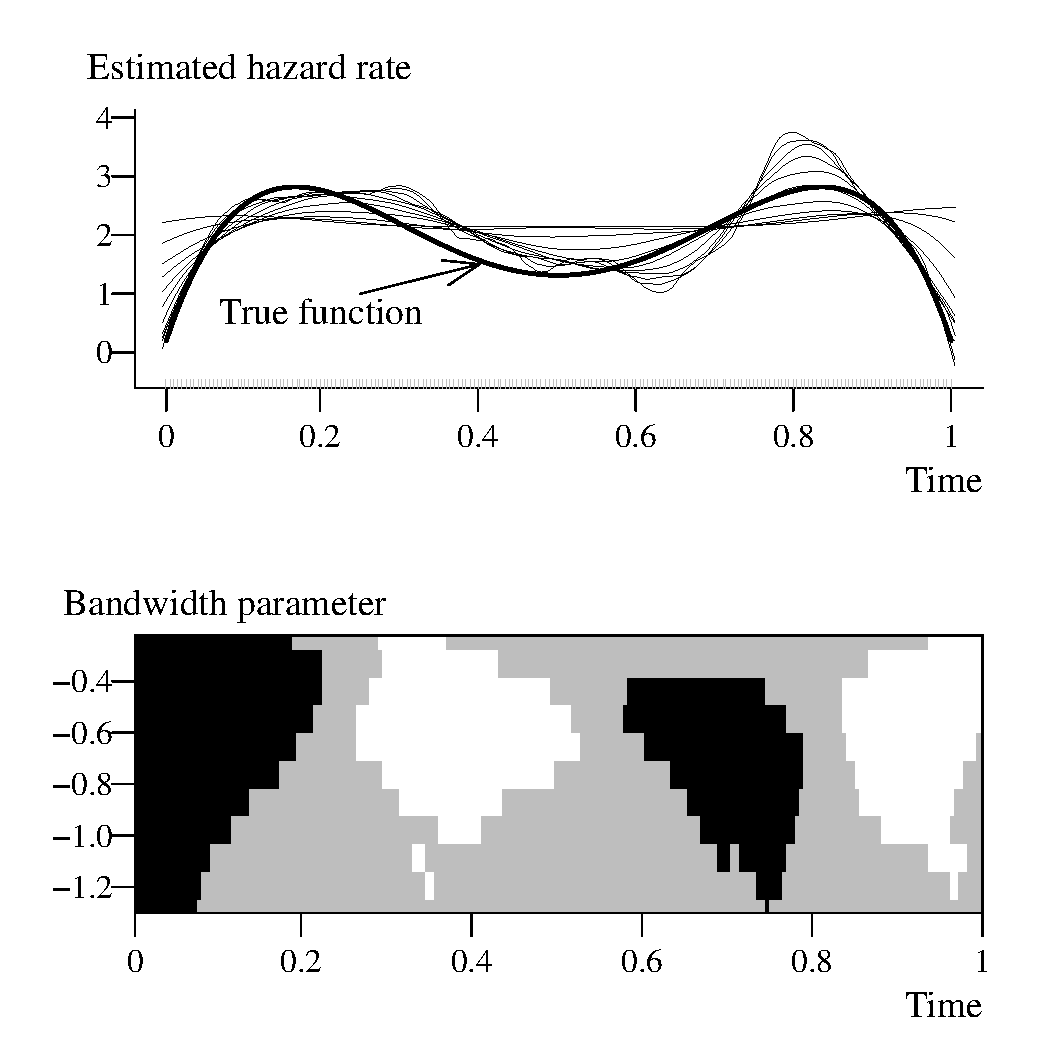
\includegraphics[width=9.5cm]{modelo6.pdf}
\caption{``SiZer'' with simulated data. From left to right, the change black, white, black, then white indicates three changes in trend, revealing two significant bumps.}\label{Fig:model2}
\end{center}
\end{figure}




\subsection{``SiZer'' for evaluating aging trends}
\noindent In this section, we take the general ideas behind SiZer methodology (Chaudhuri and Marron 1999, 2000) and adapt it to be able to inspect a specific aging property that underlies the lifetime being analyzed.

\subsection*{The family of lifetime distributions based on the hazard rate}
\noindent In this case we examine the sign of the second derivative of the TTT curve. Then we have calculated confidence intervals for $\varphi''(p)$. That is
For $0\leq p \leq 1$,
\begin{equation}\label{ci_d2phi}
\left[\widehat{\varphi}''_h(p)-q_{1-\frac{\alpha}{2}}\sqrt{{\rm Var}\left(\widehat{\varphi}''_h(p)\right)}, \ \widehat{\varphi}''_h(p)+q_{1-\frac{\alpha}{2}}\sqrt{{\rm Var}\left(\widehat{\varphi}''_h(p)\right)}\right]
\end{equation}
where $q$ is a proper quantile, and $\alpha$ the overall significance level of the tests. The derivative is significantly positive (negative) when both confidence limits are above (below) 0, and insignificant when the confidence limits bracket 0.

We can explore changes of trend of the hazard by studying the sign of the interval, and then we can establish the following classification:
\begin{itemize}
\item The IFR (DFR) family:
\noindent If the interval in \eqref{ci_d2phi} is negative (positive) we believe with a confidence of $(1-\alpha)100\%$ that the underlying lifetime is IFR (DFR)
\item The UFR family:
\noindent If the interval \eqref{ci_d2phi} is first positive and changes to negative we believe with a confidence of $(1-\alpha)100\%$  the underlying hazard is unimodal shaped.
\item The BFR family:
\noindent If the interval \eqref{ci_d2phi} is first positive and changes to negative we believe with a confidence of $(1-\alpha)100\%$  the underlying hazard is bathtub shaped.
\end{itemize}

\subsection*{More general properties}
\noindent SiZer map techniques are developed for other classes of life distributions more general than the IFR (DFR) class.
\begin{itemize}
\item The NBUE (NWUE) family of lifetime distributions.

\noindent In this case we examine the sign of the following transformation of the  TTT curve: $g(p)=\varphi(p)/p$.
\subsection*{Confidence interval for $g(p)$}
\noindent For $0\leq p \leq 1$,
\[
\left[\frac{\widehat{\varphi}_h(p)-q_{1-\frac{\alpha}{2}}\sqrt{{\rm Var}\left(\widehat{\varphi}_h(p)\right)}}{p}, \ \frac{\widehat{\varphi}_h(p)+q_{1-\frac{\alpha}{2}}\sqrt{{\rm Var}\left(\widehat{\varphi}_h(p)\right)}}{p}\right]
\]

\bigskip

\item The DMRL (IMRL) family of lifetime distributions

\noindent Este caso no estoy segura de incluirlo*****.....
\end{itemize}

\subsection{Diferent quantile}
\noindent Candidates for calculation of the quantile $q$ include:
\begin{itemize}
	\item pointwise Gaussian quantiles: $q_1(h) = q_1 = \Phi^{-1}[1-\alpha/2]$, with $\Phi$ the standard normal distribution function. 
	\item approximate simultaneous over $p$ Gaussian quantiles: based on "number of independent blocks" (Hannig and Marron, 2006), defined as
	$$
	q_2(h) = \Phi^{-1} \left[\left(1- \frac{\alpha}{2}\right)^{1/\left\{\theta(\Delta)g\right\}}\right],
	$$
	where
	$$
	\theta(\Delta) =2 \Phi \left\{ \frac{\Delta \sqrt{3 \log(g)}}{2h}\right\}-1
	$$
	$g$ is the number of pixels in a row in the SiZer Map, $\Delta$ is the distance between two succesive neighboring locations $p_0$.
	In Hannig and Marron (2006) the quantity $\theta(\Delta)$ is defined as the clustering index that measures the level of dependency between pixels. 
\end{itemize}

\subsection{Hypothesis testing based on SiZer Map}
\noindent We are firstly interested in checking whether the data are exponentially distributed. In such a case the true TTT curve coincides with the diagonal of the unit square. Let $X$ be a random lifetime, we want to test the null hypothesis 
\[
{\rm H_0 :} \ X \ {\rm follows \ Exp}(\lambda) \ {\rm distribution,\ for \ some} \lambda >0,
\]
against general alternatives based on a sample $X_1, X_2,\ldots, X_n$ of independent copies of $X$.
To solve the problem we propose a new procedure based on the TTT-transform and that uses the SiZer tool. In other words, we set the following hypothesis testing problem:
\begin{eqnarray} \label{test_exp}
\nonumber &&{\rm H_0 :} \ \varphi_X''(p)= 0, {\rm for \ all \ } p \in (0,1) \\
&&{\rm H_1 :} \ \varphi_X''(p)\neq 0, {\rm for \ some \ }  p \in (0,1)
\end{eqnarray}
We can rewrite the hypotheses in \eqref{test_exp} in SiZer map language, then the null hypothesis is equivalent to assert that the underlying map to the true distribution is completely purple. We will call this one the $true$ map. We will decide to reject the null hypothesis in case that the SiZer map based on the $empirical$ map (referred as  displayes) a percentage of non purple pixels above a pre-specified level. As usual we will refer to this level the type I error probability, and denote it as $\alpha$. This value is commonly taken as $\alpha=0.05$. 

We summarize the steps of our proposal in the following algorithm.
\subsubsection*{Algorithm 2. Testing exponentiality $vs.$  aging trend} 
\begin{enumerate}
\item[Step 1.] Compute the sample mean $\bar{X}$ and define $\bar{X}_i=X_i/\bar{X}$, for $ i=1,2,\ldots,n$;
\item[Step 2.] Generate  $M$ bootstrap samples as explained in Algorithm 1, and construct the corresponding ${\bf X}^*$, matrix. 
\item[Step 3.] Construct $M$ empirical SiZer maps for the second derivative as explained in Section.... One for each bootstrap sample of each column of matrix ${\bf X}^*$;
\item[Step 4.] Compare each $empirical$ map with the $true$ map pixel by pixel, and count the total number of pixels where the color in the generated $empirical$ map is not the same as in the $true$ map. Define a binary function $\delta$ taking value 1 when the corresponding empirical map reports one or more than one non-purple pixels;
\item[Step 5.] Define the bootstrap $p$-value as $\sum_{m=1}^M \delta_m /M$
\item[Step 6.] Reject the null hypothesis when $p$- value lower than $\alpha$
\end{enumerate}
 %p-valor: Para una muestra concreta, se trata de calcular la probabilidad de que bajo la hipótesis nula obtengamos una muestra peor que la que tenemos.  Este problema lo tenemos que (podemos) implementar basándonos en unos datos reales
%6.1 Creamos el EmpiMap basado en los datos y lo comparamos con el TrueMap. Calculamos la proporción de pixels que no coinciden con lo que queremos.
%6.2 Generamos una muestra bootstrap con reemplazamiento a partir de los datos
%6.3 Construimos el EmpiMap* bootstrap y lo comparamos con el TrueMap igual que en el punto 6.1
%6.4 Repetimos los puntos 6.2-6-3 R=1000 veces
%El p-valor lo podemos definir como la proporción de EmpiMap* (bootstrap) que dieron un resultado peor que el de EmpiMap basado en los datos.
\newpage
%%%%%%%%%%%%%%%%%%%%%%%%

\section{Simulations}

\section{Real data examples}

\section{Concluding remarks}

The aim of this paper has been to .....
\newpage
\begin{thebibliography}{}
% Los años al final de la referencia
\bibitem{ABGK1993}

\bibitem{ABN08} Arnold, B.C., Balakrishnan, N. and Nagaraja, H.N. A First Course in Order Statistics. Classics in Applied Mathematics New York: Willey. (2008)

\bibitem{BC75} Barlow, R.E. and Campo, R. Total time on test processes and applications to failure data analysis. In Reliability and Fault Tree Analysis, Edited by: Barlow, R.E., Fussell, J. and Singpurwalla, N.D. (1975) 451–481

\bibitem{BD72} Barlow and Doksum (1972) Isotonic test for convex ordering. Procedings of the 6$th$ Berkeley Symposium on Mathematical Statistics and Probability, Vol. 1,pp. 293--323, University of California Press

\bibitem{BP75} Barlow, R. E. and F. Proschan (1975). Statistical theory of reliability and life testing. Holt,
Rinehart and Winston.

\bibitem{BK84} Bergman, B. and Klefsjö, B. The Total Time on Test Concept and Its Use in Reliability Theory. Operations Research, 32(3), Reliability and Maintainability, (1984) 596--606.

\bibitem{CH99} Chaudhuri, P. and Marron, J.S. SiZer for Exploration of Structures in Curves. Journal of the American Statistical Association, 94(447), (1999)  807--823.

\bibitem{CM02} Chaudhuri, P. and Marron, J.S. Curvatuve vs. Slope Inference for Features in Nonparametric Curve Estimates. (2002) 

\bibitem{HM2006} Hannig, J. and Marron, J.S. Advanced Distribution Theory for SiZer. Journal of the American Statistical Association, 101(474) (2006) 484--499.

\bibitem{HE2000} Hutson, A.D., and Ernst, M. (2000) The exact bootstrap mean and variance of an L-estimator, J.R. Statist. Soc B. Vol. 62, Part 1, pp. 89--94.
\bibitem{Nair2010} Nair {\it et al.} (2010)

\bibitem{U} Unnikirishnan Nair, N., Sankaran, P.G. and Balakrishnan, N. () Quantile-Based Realiability Analysis. 

\end{thebibliography}


\end{document}
